On this chapter it will be introduced an algorithm for land cover classification using the parameters estimated from the temporal decorrelation. The algorithm will be based on the Random Forest classification algorithm and it will be discussed the training and validation method used for this algorithm. The results will be compared with external reference for the classification area over Germany.
After that this algorithm will be used to perform a land cover classification over the Amazon Rainforest and it will be shown the overall performance with the PRODES classification map.

\section{The Germany Classification}

Out of the 7 stacks available (described on section 4.5) for the Germany dataset, the first 6 were used as training data for the Random Forest model and the last one was used for testing and model evaluation.

\subsection{Parameter Estimation}
For the first step of the analysis the algorithm from the formula [3.2] must be used. Using the stacks 1-6 for the Germany dataset for parameter estimation, combined with the Corine Landcover map as classification reference it is possible to evaluate the multilooked backscatter $\hat{\gamma}^0$ for different classes (artificial surfaces, forests and non-forest areas) and then perform the exponential fit of the temporal correlation $\hat{\rho}_{temp}$ extracting the parameters $\hat{\rho}_{LT}$ and $\hat{\tau}$.

For the exponential fitting it was used the temporal decorrelation models previously mentioned on this work - shown in formulas \ref{decor1}, \ref{decor2}, \ref{decor3} and \ref{decor_final}. For the exponential fitting it was used a set of 3000 observations (1000 for each class) that were randomly selected from the data set. Then, the exponential fit was performed and it was calculated the mean square error (MSE) between the measurements and the model and the mean square error standard deviation. The table below shows this value for the 4 models that were introduced on this work.

\begin{table}[H]
    \centering
    \begin{tabular}{c|c|c}
    \hline
     Model&Mean MSE& MSE standard deviation  \\
     \hline
     1&0.047&0.012\\
     2&0.155&0.044\\
     3&0.006&0.008\\
     4&0.005&0.007\\
     \hline
    \end{tabular}
\caption{Mean MSE and MSE standard deviation using 3000 samples (1000 for each class). Four different models were considered: Model 1 is given by equation (2.3), model 2 is given by equation (2.4), model 3 is given by equation (2.5) and model 4 is given by equation (2.6) }
\label{tabelamse}
\end{table}

From the table \ref{tabelamse} it is clear that the model 4 has superior performance and why it was used as the model for this work.

After the parameters of interest were extracted from the training data, it was computed the normalized histograms for each class. The principle is that if the probability density functions for the classes have little overlap then it should be easy to infer which pixel belongs to each class, while if the probability density functions have a big overlap then it should be hard to infer to which class each pixel corresponds to. 

On \figref{fig:normalized_histograms}, it is possible to visualize the histograms for each parameter for each class and the graph of the temporal decorrelation for the fitted parameters.

\begin{figure}[H]
    \centering
    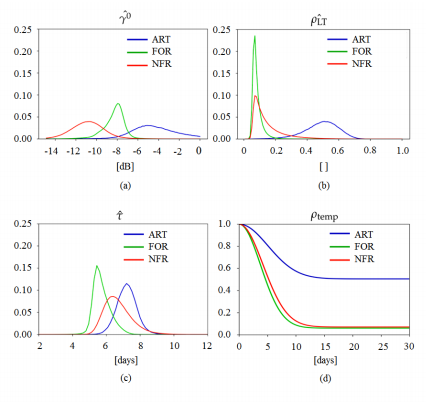
\includegraphics{Cap4/histogramas.png}
    \caption{(a)Normalized histograms for the backscatter $\hat{\gamma}^0$. (b) Normalized histograms for $\hat{\rho}_{LT}$. (c) Normalized histograms for $\hat{\tau}$. (d) Exponential model for the temporal decorrelation of each class using the mean values of backscatter, long term coherence and decay factor }
    \label{fig:normalized_histograms}
\end{figure}

From the image above it is seen from both the histograms for the Forest (FOR) and for the non-forest areas (NFR) that the classes are highly correlated and that the artificial surface class (ART) should be relatively easy to identify (specially considering the long term coherence parameter).

\subsection{Classification and Evaluation}
In order to confirm that the estimated parameters provide valuable information for the land cover classification it is proposed three different cases, characterized by different input information for the Random Forest classifier:

\begin{enumerate}
    \item  $\hat{\gamma}^0$ and $\theta_{inc}$
    \item  $\hat{\tau}$, $\hat{\rho}_{LT}$ and $\theta_{inc}$
    \item $\hat{\gamma}^0$, $\hat{\tau}$, $\hat{\rho}_{LT}$ and $\theta_{inc}$
\end{enumerate}

For the Random Forest classifier it is important to tune two hyperparameters for the training algorithm: The minimum number of samples in a leaf node ($leaf_{size}$) and the number of different trees used for classification ($n_{est}$). Usually the bigger the numbers for both parameters the better the classification (at the expense that more time will be used for both training and classifying the data). It is worth mentioning that if the values increase too much then the overall accuracy starts to decrease due to overfitting of the model. For both parameters the value of $50$ was used - this was chosen based on the fact that increasing this value much further showed no significant performance improvement.

For the three different cases the case 3 showed the best performance for classification as expected. On the image below it can be seen the classification that was performed for the Germany area using this method.

\begin{figure}[H]
    \centering
    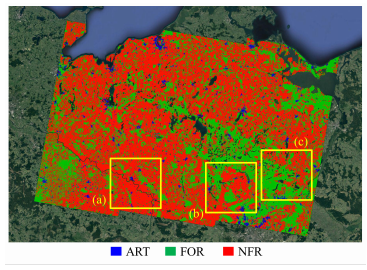
\includegraphics{Cap4/classificacao3.png}
    \caption{Classification map for the stack 7 of Sentinel-1 Data overlaped with Google Earth. Blue represents Artificial Surfaces, Green represents Forest areas and Red represents Non-Forest Areas}
    \label{fig:classification_germany}
\end{figure}

For the comparison of the different classification models it was chosen three different patches on the image and it was performed the classification for these patches using the three different cases(patches shown in \figref{fig:classification_germany}. It was also performed an overall classification where 2 million pixels were randomly selected from the area and classified. The results were obtained by comparing the model classification results with the Corine Land Cover Map.

The results for these comparisons can be seen on the table \ref{tab:class_accuracy_rondonia}

\begin{table}[H]
    \centering
    \begin{tabular}{c|c|c|c|c}
    \hline
         input case&patch a&patch b&patch c& overall  \\
         \hline
         case 1 & 76.02\%&79.93\%&76.86\%&88.73\%\\
         case 2 &79.30\%&77.98\%&71.3\%&78.77\%\\
         case 3&83.28\%&86.84\%&82.9\%&91.85\%\\
         \hline
         
    \end{tabular}
    \caption{Classification Accuracy for the three patches (a), (b) and (c) from Figure (4.2) and the Overall Accuracy (2 millions pixels were randomly chosen). It was performed classification used the three inputs cases previously specified.}
    \label{tab:class_accuracy_corine}
\end{table}

From the table above it is clear that this temporal decorrelation method indeed extracts valuable information for the land cover classification.

Now this method is going to be applied in a SENTINEL1 dataset which was acquired over the Amazon Rainforest.

\section{The Amazon Rainforest Classification}
For the Amazon Rainforest dataset it is available 12 stacks (defined on section 4.5) which were split between training and validation datasets. For the training dataset the stacks 1, 2, 3, 4, 5, 10, 11, 12 and the remaining stacks were used for the validation of the parameter. 

For the training of the Random Forest 5 million pixels were randomly extracted from the training dataset for each class (except for the Artificial Surface since there is a low amount of pixels for the training, for this case standard data augmentation methods were used). 

On \figref{fig:results_rondonia}, it can be seen the results of the classification in comparison with the PRODES reference map. It is worth mentioning that the PRODES reference map also includes the cuts that were made between 2017 and 2019.

\begin{figure}[H]
    \centering
    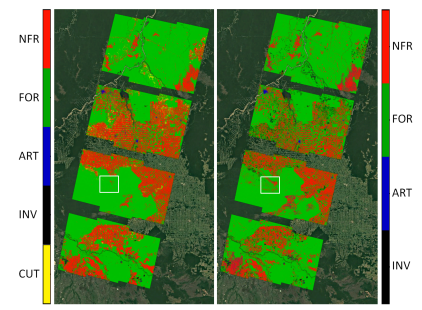
\includegraphics{Cap4/classificacaoamazon.png}
    \caption{Comparison between the REF reference (left), with in yellow the clearcuts (CUT) marked by
PRODES between 2017 and 2019 and the classification result using interferometric parameters as additional input for the Random Forest.}
    \label{fig:results_rondonia}
\end{figure}

On the table \ref{tab:class_accuracy_rondonia} it can be also seen the Overall accuracy and the average accuracy for the validation dataset stacks.

\begin{table}[H]
    \centering
    \begin{tabular}{c|c|c|c|c|c}
    \hline
         &\textbf{Class}&\textbf{Stack 6}&\textbf{Stack 7}& \textbf{Stack 8} & \textbf{Stack9}\\
         \hline
         pixels&ART&10060&34890&6009&1054\\
         pixels&FOR&14626324&7846234&9822268&10087671\\
         pixels&NFR&1655335&6194973&4193972&4280135\\
         \hline
         \textbf{Case}&\textbf{Metric}&\textbf{Stack 6}& \textbf{Stack 7} & \textbf{Stack 8} & \textbf{Stack 9} \\
         \hline
         &\textbf{OA}&0.8848&08250&0.8503&0.8484\\
         &\textbf{AA}&0.6105&0.8164&0.8050&0.7195\\
         \hline
    \end{tabular}
    \caption{Number of pixels for each class used for validating results with Prodes Classification Map and Overall Accuracy and Average Accuracy for the four swaths acquisitions. Each Swath is associated with a Stack.}
    \label{tab:class_accuracy_rondonia}
\end{table}